\chapter{Mindmap}
\begin{figure}[!ht]
  \centering
  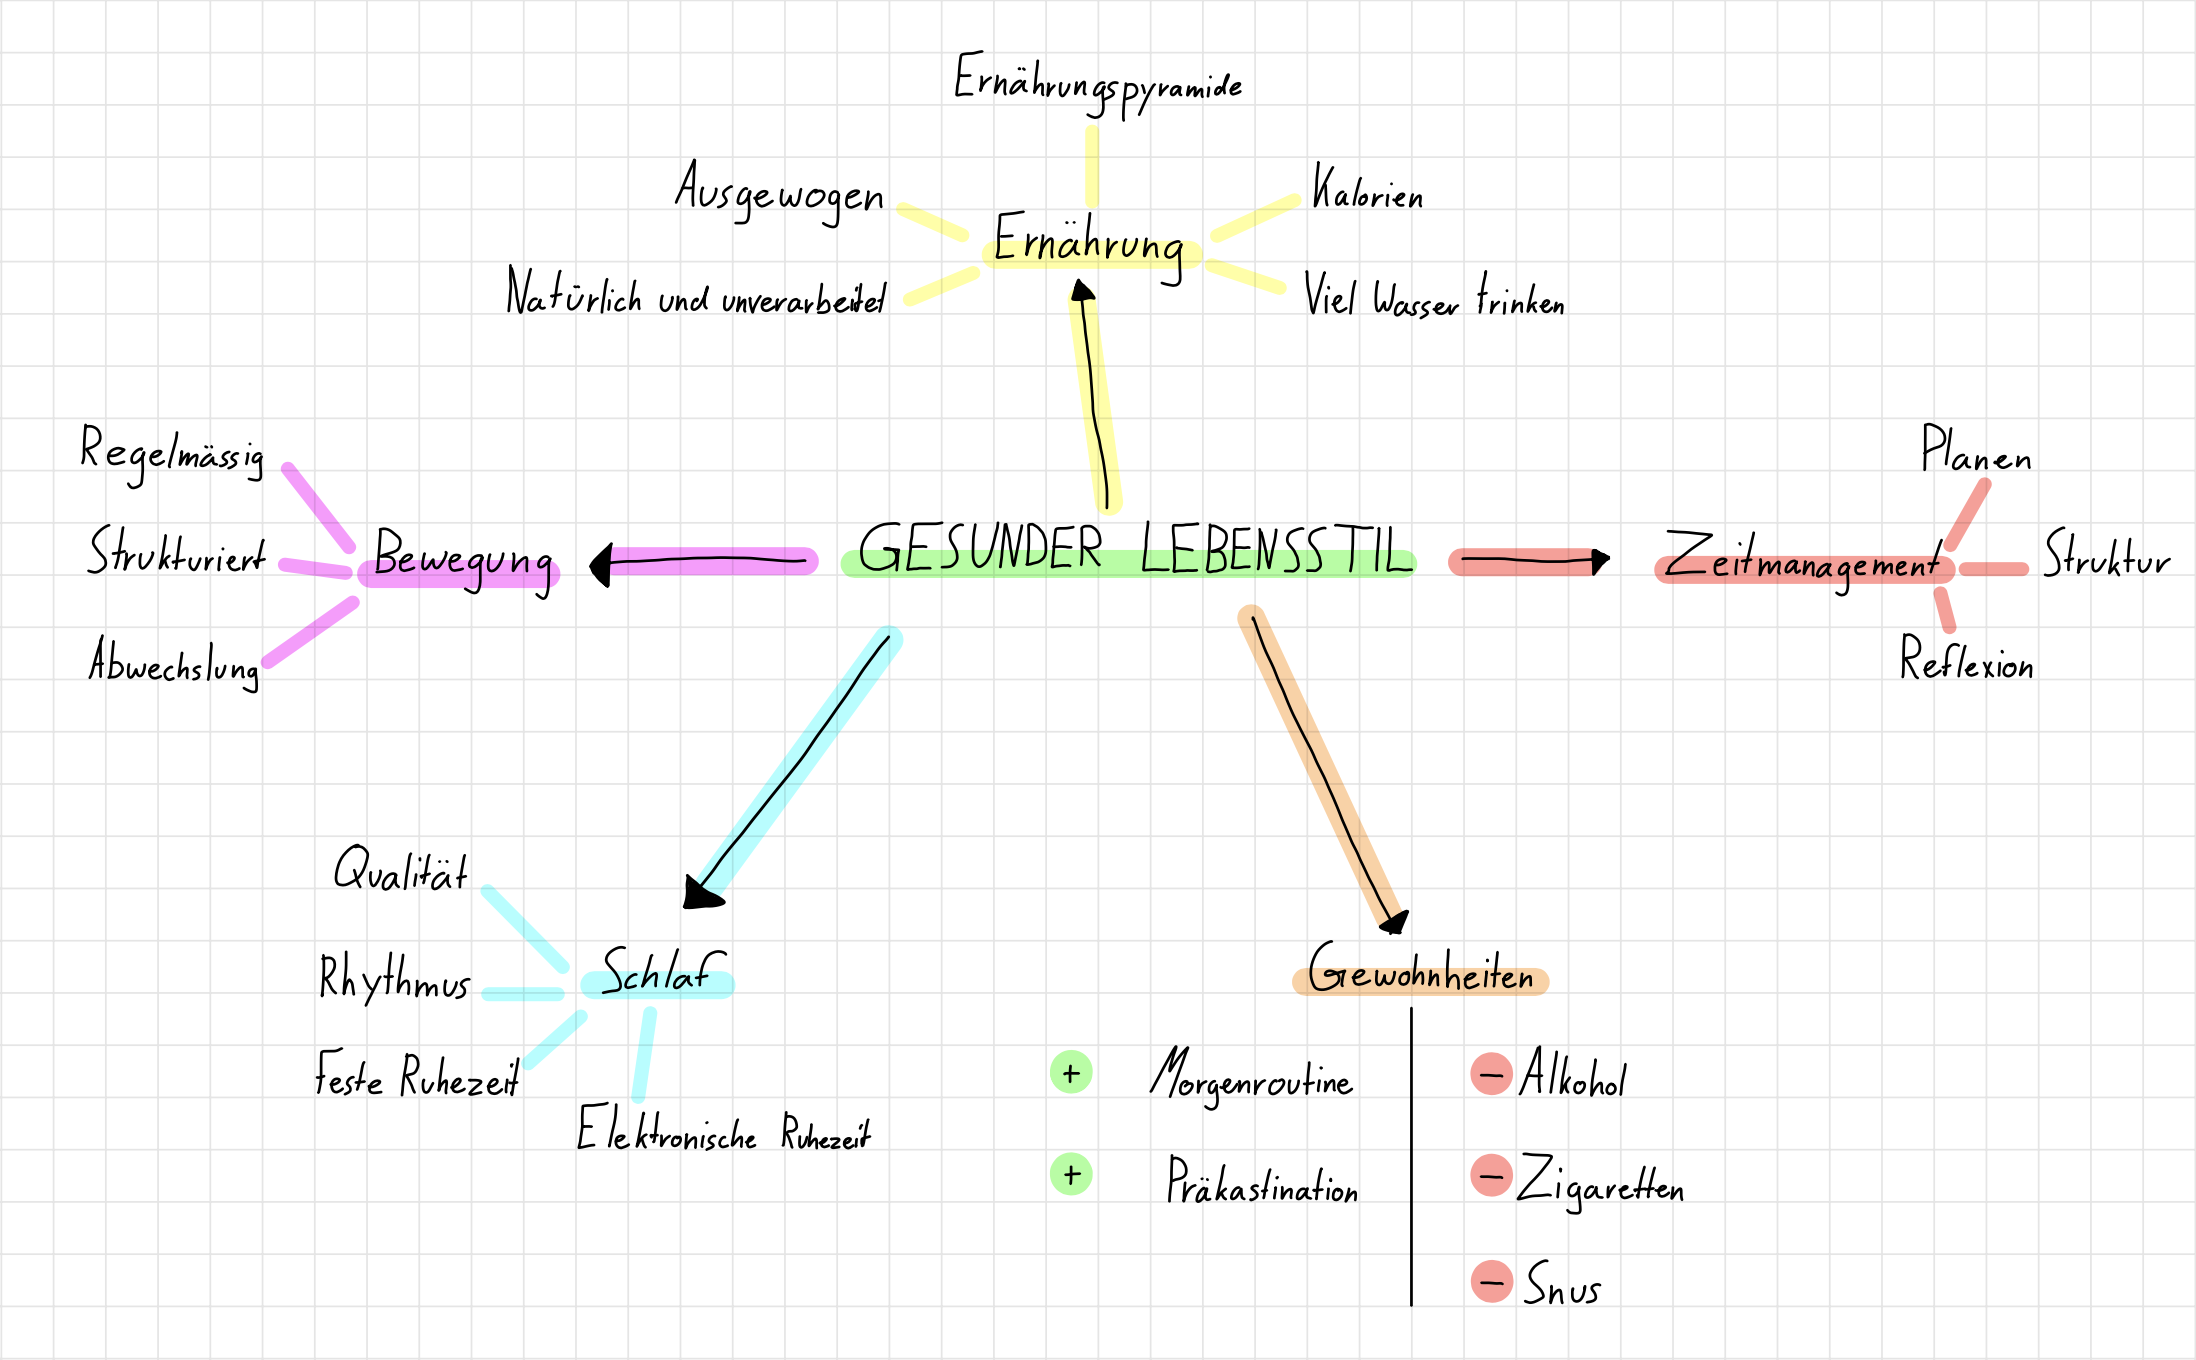
\includegraphics[width=.9\linewidth]{./images/mindmap.png}
  \caption[Ein von uns digital erstelltes Mindmap]{Wasserfall Modell}
  \label{fig:wasserfall}
\end{figure}
Wir haben uns zusammengesetzt und überlegt, was alles zu einem gesunden Lebensstil gehört.
\newline
Dafür haben wir ein Mindmap erstellt, welche unsere Überlegungen widerspiegelt. Dabei haben wir fünf Themen gewählt, welche unserer Meinung nach die wichtigsten für einen gesunden Lebensstil sind. Diese Themen sind zum einen die Bewegung, zum Anderen die Ernährung, das Zeitmanagement, die Gewohnheiten und ebenfalls der Schlaf.
\newline
Zu diesen Punkten haben wir schlussendlich einige Ideen gesammelt, welche unserer Meinung nach wichtig waren.
\begin{enumerate}
  \item Bei der Bewegung haben wir als wichtige Unterpunkte die Regelmässigkeit, die Strukturierung und die Abwechslung. Unsere Überlegungen waren, dass wir eine Routine hereinbringen und uns dabei mehrmals wöchentlich auf eine sportliche Art bewegen und dies auch Abwechslungsreich gestalten. Damit meinen wir, dass man nicht immer das gleiche machen muss, wie z.B. Krafttraining. Sondern ebenfalls auch Ausdauertraining oder je nachdem auch andere Arten von Training zur Förderung der Bewegung. Zudem setzt man mehr Muskelreize, wenn das Training auf verschiedene Art die Muskulatur beansprucht. Das sorgt für eine gute und qualitativ hochwertige Muskulatur.
  \item Bei der Ernährung haben wir fünf wichtige Unterthemen gewählt: Natürlich und unverarbeitet, Ausgewogen, Ernährungspyramide, Kalorien und viel Wasser trinken. Dabei haben wir uns gedacht, dass man möglichst wenig verarbeitete Produkte essen sollte und stattdessen lieber auf unverarbeitete Produkte setzt. Ein Beispiel dafür wäre ein Wienerli und Pouletbrust. beides ist Fleisch, jedoch ist das eine verarbeitetes Fleisch und das andere unverarbeitet und mit der Verarbeitung wird das Produkt ungesünder. Es ist auch sehr wichtig, dass die Ernährung ausgewogen ist, was heisst, dass sie vielseitig und von allem etwas dabei haben sollte. Ebenfalls kann man sich auch nach der Ernährungspyramide richten, welche vorgibt, wie viel Lebensmittel man konsumieren sollte um sich ausgeglichen und gesund zu ernähren.Auch die Kalorienanzahl ist wichtig, denn gesund ist nicht gleich kalorienarm. Es gibt viel gesundes, was aber sehr viele Kalorien hat. Trotzdem sollte man schauen, dass man seine Tagesration an Kalorien einteilt und nicht zu viel einnimmt. Zum Schluss haben wir die simpelste Sache und das wäre viel Wasser trinken. Dafür sollten andere Getränke, wie zum Beispiel Süssgetränke möglichst nicht konsumiert werden.
  \item Als nächster Punkt haben wir das Zeitmanagement mit den Unterthemen Planen, Struktur und Reflexion. Bei der Umsetzung des Zeitmanagement ist es wichtig, dass wir uns einen Plan machen. Das kann ein wöchentlicher oder sogar ein täglicher Plan sein. So bringen wir auch eine gerade Struktur in den Alltag. Mit einer Reflexion des Tages wollen wir schauen, wie es uns erging, was wir gemacht haben usw. 
  \item Kommen wir zu den Gewohnheiten. Diese haben wir in positive und negative unterteilt. Schlechte Gewohnheiten wären: der Alkoholkonsum, der Zigarettenkonsum und der Snus Konsum. Diese gilt es auf jeden Fall zu reduzieren, da sie sehr ungesund sind und nicht zu einem gesunden Lebensstil dazu gehören. Im Gegensatz zu dem gibt es auch noch die positiven Gewohnheiten. Bei diesen haben wir die Morgenroutine und Präkastination genommen. Eine Morgenroutine ist sehr wichtig, da wir so eine bessere Struktur in unseren Alltag bringen und dadurch einen guten Start in den Tag haben werden. Die Präkastination, was soviel heisst, wie nicht ständig die Aufgaben aufschieben, ist auch eine sehr gute Gewohnheit. Wenn wir Dinge gerade erledigen und sie nicht noch lange aufschieben, haben wir ein besseres Zeitmanagement und kommen so nicht in Stress. 
  \item Beim Schlaf haben wir die Qualität, den Rhythmus, eine feste Ruhezeit und eine elektronische Ruhezeit. Mit Qualität wird gemeint, dass das Bett zum Beispiel nur zum Schlafen verwendet wird und ansonsten man nicht im Bett liegen sollte. Dies ergibt einen qualitativ hochwertigeren Schlaf. Ebenfalls sollte  beachtet  werden, dass man einen gewissen Rhythmus hat und nicht immer zu anderen Zeiten ins Bett geht und aufsteht. Dies verbessert die Schlafqualität noch einmal. Zudem sollte eine feste Ruhezeit festgelegt werden. Diese Zeit wird als Minimale festgelegt, welche wir pro Nacht schlafen sollten, damit unser Körper erholt ist. Auch ist eine elektronische Ruhezeit wichtig. So kann sich der Körper schon vorher entspannen und wird nicht vom Blaulicht das Smartphones oder eines anderen elektrischen Geräts wach gehalten.
\end{enumerate}